\documentclass[]{IEEEtran}

\title{Modellazione e Sintesi di un Moltiplicatore Floating-point Single Precision}
\author{Enrico Sgarbanti - VR446095}

\usepackage{graphicx}
\usepackage{subfig}
\usepackage{wrapfig}
\usepackage{hyperref}
\usepackage[italian]{babel}
\usepackage[utf8]{inputenc}

\begin{document}
\maketitle



\begin{abstract}
    Questo documento mostra la realizzazione di un moltiplicatore in virgola mobile a precisione singola realizzato in VHDL, Verilog e SystemC ed un componente che permetta di eseguire due moltiplicazioni in parallelo. Il tutto è accompagnato da testbench, sintesi dei componenti VHDL e verilog ed un confronto con l'High-level-Synthesis di un moltiplicatore scritto in c++.
\end{abstract}



\section{Introduzione}
Il progetto consiste nella realizzazione in hardware di un sistema che utilizzi due moltiplicatori in virgola mobile a precisione singola, secondo lo standard IEEE754, per eseguire due moltiplicazioni in parello. Esso deve essere sintetizzabile sulla FPGA ``xc7z020clg400-1'' che possedendo solo 125 porte I/O, obbliga a serializzare input e output.
\\Il sistema è stato realizzato in diversi linguaggi al fine di scoprire le differenze tra i vari linguaggi utilizzabili per la descrizione del hardware e capirne i pro e contro. I risultati sono stati poi analizzati e confrontati con quelli ottenuti dall'high level syntesis del codice in c++.
\\L'approccio utilizzato è bottom-up, cioè si è partiti dal moltiplicatore per poi arrivare al top level. L'implementazione è preceduta dall'analisi dei requisiti e dalla stesura della EFSM, cioè la parte più importante in quanto è dove viene tradotto l'algoritmo, descritto il flusso e scelti i vari segnali intermedi necessari. Una buona EFSM permette di evitare di scrivere varie righe di codice per poi accorgersi in simulazione che qualcosa non funziona.
\\Ci si aspetta che la versione RTL sia significativamente più performante di quella con l'high level syntesis e che il sistema occupi una minima parte della FPGA in quanto molto piccolo.



\section{Background}

\subsection{Progettazione hardware}
Per la realizzazione di componenti hardware si possono utilizzare diverse tecniche e linguaggi.
\\Un primo approccio è descrivere i componenti a livello RT utilizzando linguaggi di descrizione del hardware (\textbf{HDL}) come VHDL e Verilog. Un HDL è un linguaggio specializzato per la descrizione della struttura e del comportamento di circuiti elettronici, in particolare circuiti logici digitali, e la loro analisi e simulazione. Permette inoltre la sintesi di una descrizione HDL in una netlist (una specifica di componenti elettronici fisici e il modo in cui sono collegati insieme), che può quindi essere posizionata e instradata per produrre l'insieme di maschere utilizzate per creare un circuito integrato\cite{HDL}.
\\Un secondo approccio è descrivere le funzionalità del componente con linguaggi più ad alto livello come C, C++ o SystemC\cite{SystemC} e fare High Level Syntesis (\textbf{HLS}) per ottenere una descrizione dell'hardware a livello RT\cite{HLS}.
\\Entrambi gli approcci hanno vantaggi e svantaggi. In particolare HLS riduce i tempi, ma la descrizione hardware generata sarà meno ottimizzata rispetto a quella che si potrebbe ottenere usando un HDL.


\subsection{IEEE 754 single-precision binary floating-point format}
Lo standard 754\cite{IEEE754} è la rappresentazione più comune per i numeri reali. Esso definisce il \textbf{formato} per la rappresentazione dei numeri in virgola mobile (compreso $\pm 0$ e i numeri denormalizzati (o subnormali); gli infiniti e i NaN, "not a number"), ed un set di operazioni effettuabili su questi \cite{IEEE754Wiki}.
\\La rappresentazione in virgola fissa ha una "finestra <" di rappresentazione che gli impedisce di rappresentare sia numeri molto grandi che molto piccoli. Invece la rappresentazione in virgola mobile utilizza una sorta di "finestra scorrevole" di precisione adeguata alla scala del numero permettendogli di massimizzare la precisione su entrambe le estremità della scala \cite{IEEE754Online}.
\\In particolare la versione a precisione singola dello standard IEEE754 descrive il numero con 32 bit: 1 bit per segno (sign), 8 bit per l'esponente (exp) e 23 bit per la mantissa (mant).
\\Per la \textbf{codifica} in numero binario normalizzato:
\begin{itemize}
    \item Il bit del segno \textit{sign} è 1 se il numero è negativo 0 altrimenti.
    \item Si converte il numero in binario in virgola fissa.
    \item Si sposta la virgola a sinistra o destra fino ad avere un numero nella forma $1.x \cdot 2^{E}$.
    \item I bit della mantissa \textit{mant} sono la parte a destra della virgola, con zeri a destra fino a riempire i 23 bit. Il bit a 1 a sinistra della virgola è omesso.
    \item I bit dell'esponente \textit{exp} sono uguali a $127+E$ dove 127 è il \textit{bias} di questo standard per la versione a precisione singola.
\end{itemize}
Per la \textbf{decodifica} del numero binario normalizzato: $$(-1)^{sign}\cdot 2^{(exp-127)} \cdot (1 + \sum_{i=1}^{23}b_{23-i}\cdot 2^{-i})$$
\\Ci sono però dei casi particolari rappresentati in modo diverso:
\begin{itemize}
    \item \textbf{zero:} è rappresentato mettendo tutti i bit di esponente e mantissa a 0.
    \item \textbf{infinito:} è rappresentato mettendo tutti i bit dell'esponente a 1 e quelli della mantissa a 0.
    \item \textbf{NaN:} presentano tutti i bit dell'esponente a 1, ma non hanno tutti i bit della mantissa a 0. Essi vengono utilizzati per rappresentare un valore che non rappresenta un numero reale. Esistono due categorie di NaN:
          \begin{itemize}
              \item \textbf{Quiet NaN:} esso ha il bit più significativo della mantissa a 1. Indica un valore indeterminato genarato da operazioni aritmetiche il cui risultato non è matematicamente definito.
              \item \textbf{Signal NaN:} esso ha il bit più significativo della mantissa a 0. Indica un valore non valido. Può essere utilizzato per segnalare eccezioni causate da operazioni o per indicare variabili non inizializzate .
          \end{itemize}
    \item \textbf{Numeri denormalizzati:} presentano tutti i bit dell'esponente a 0, ma non hanno tutti i bit della mantissa a 0. Essi sono decodificati in modo differente dai numeri normalizzati: $$(-1)^{sign}\cdot 2^{(-126)} \cdot (0 + \sum_{i=1}^{23}b_{23-i}\cdot 2^{-i})$$. Ovvero il bit omesso vale 0 anzichè 1 e l'esponente effettivo del numero vale sempre -126  \cite{IEEE754Online}.
\end{itemize}

\begin{figure}[!htb]
    \centering
    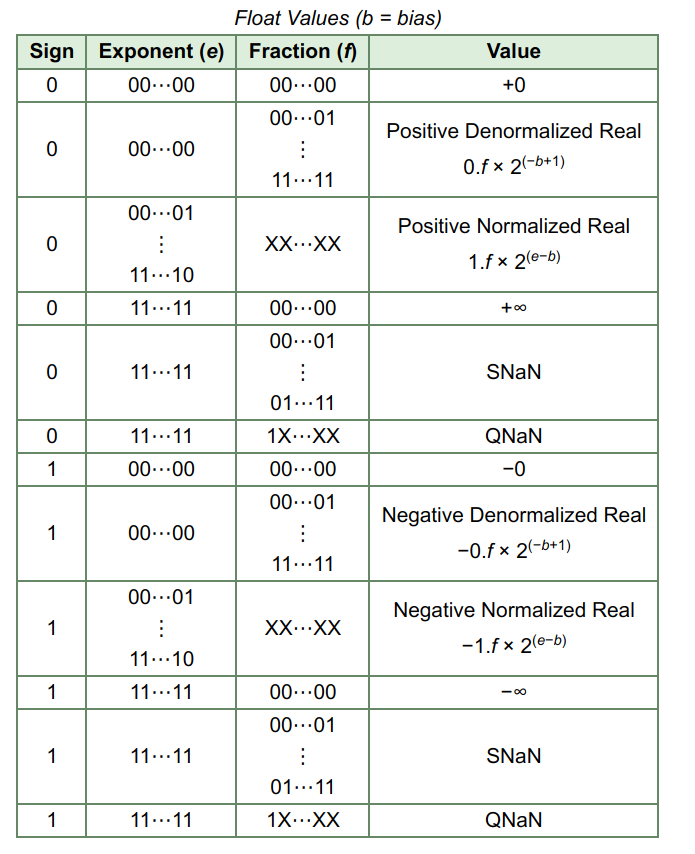
\includegraphics[width=0.9\linewidth]{figures/codifica}
    \caption{IEEE 754 casi possibili. (Steve Hollasch, Online \cite{IEEE754Online})}
    \label{fig:IEEE_ENCODING}
\end{figure}



\section{Metodologia applicata}

\subsection{Struttura progetto}
\begin{itemize}
    \item \textbf{cpp/} contiene il file\textbf{multiplier.cpp} dove è presente una funzione che esegue la moltiplicazione in c++.
    \item \textbf{SystemC/}
          \begin{itemize}
              \item \textbf{Makefile:} tool per la compilazione automatica del progetto. Richiede che la variabile d'ambiente SYSTEMC\_HOME contenga il path alla libreria di SystemC.
              \item \textbf{include:} contiene gli headers del progetto. Qui sono definite tutte le porte, segnali ed enumerazioni dei vari componenti.
              \item \textbf{src:} contiene i file sorgenti del progetto..
              \item \textbf{bin:} contiene l'eseguibile \textbf{double\_multiplier\_RLT.x} (generato dopo la compilazione) e la simulazione \textbf{wave.vcd} (generato dopo l'esecuzione dell'eseguibile).
              \item \textbf{obj:} contiene i file oggetto (generati dopo la compilazione).
          \end{itemize}
    \item \textbf{VHDL\_verilog/}
          \begin{itemize}
              \item \textbf{stimuli/} contiene gli script TCL usati per dei test.
              \item \textbf{waves/} contiene i file per visualizzare le simulazioni come negli screenshot.
              \item \textbf{constrains/} contiene i vincoli per la sintesi.
              \item \textbf{double\_multiplier} file Verilog del top level del sistema.
              \item \textbf{verilog\_multiplier} file Verilog del moltiplicatore IEEE754.
              \item \textbf{vhdl\_multiplier} file VHDL del moltiplicatore IEEE754.
              \item \textbf{testbench} file Verilog contenente il testbench.
          \end{itemize}
\end{itemize}


\subsection{Procedimento}
Per prima cosa è stato studiato lo standard IEE754 ed è stato definito l'algoritmo ad alto livello per la moltiplicazione. Dopodichè è stata realizzata la EFSM di \textit{double\_multiplier} e \textit{double\_multiplier}.
\\A questo punto si è passati all'implementazione su Vivado\cite{Vivado} partendo con un approccio bottom-up dal \textit{multiplier} per poi passare al \textit{double\_multiplier} e infine al \textit{testbench} tutti scritti in Verilog. È stato scelto questo linguaggio per realizzare le varie componenti in quanto ritenuto più semplice da utilizzare e con una sintassi molto più chiara del VHDL. Ogni componente è stato testato con uno script TCL e in seguito con il testbench. Verificata la correttezza del sistema con due moltiplicatori Verilog si è passati a scrivere \textit{multiplier} anche in VHDL ed è stato aggiunto al testbench il confronto fra i valori ottenuti dai due componenti.
\\In seguito è stato riscritto tutto in SystemC dove è stato fatto anche un testbench con numeri random.
\\Infine è stata fatta l'high level syntesis da un semplice codice c++ per confrontare i risultati ottenuti.


\subsection{Vincoli ed Architettura}
Il progetto presenta diversi vincoli:
\begin{itemize}
    \item Il \textit{multiplier} deve essere scritto in VHDL, Verilog e SystemC.
    \item Gli operandi e il risultato devono essere a 32 bit.
    \item I due componenti devono essere sintetizzabili sulla FPGA ``xc7z020clg400-1'' la quale ha a disposizione solo 125 porte.
\end{itemize}
Per far fronte al limite delle porte logiche è stato necessario serializzare input e output. Vengono quindi utilizzati gli stessi 32 bit per il risultato e altri 64 bit per le due coppie di operandi.
\\I vari componenti comunicano fra loro grazie al protocollo di \textit{handshake}. Con \textit{ready} uguale a 1 si attiva il componente, il quale quando avrà finito metterà \textit{done} uguale a 1.
\\L'architettura con VHDL e Verilog è mostrata in figura \ref{fig:Architettura}. Quella per SystemC è analoga.
\\I segnali intermedi sono stati omessi da questa figura, ma vengono descritti nelle sezioni successive.
\begin{figure}[!htb]
    \centering
    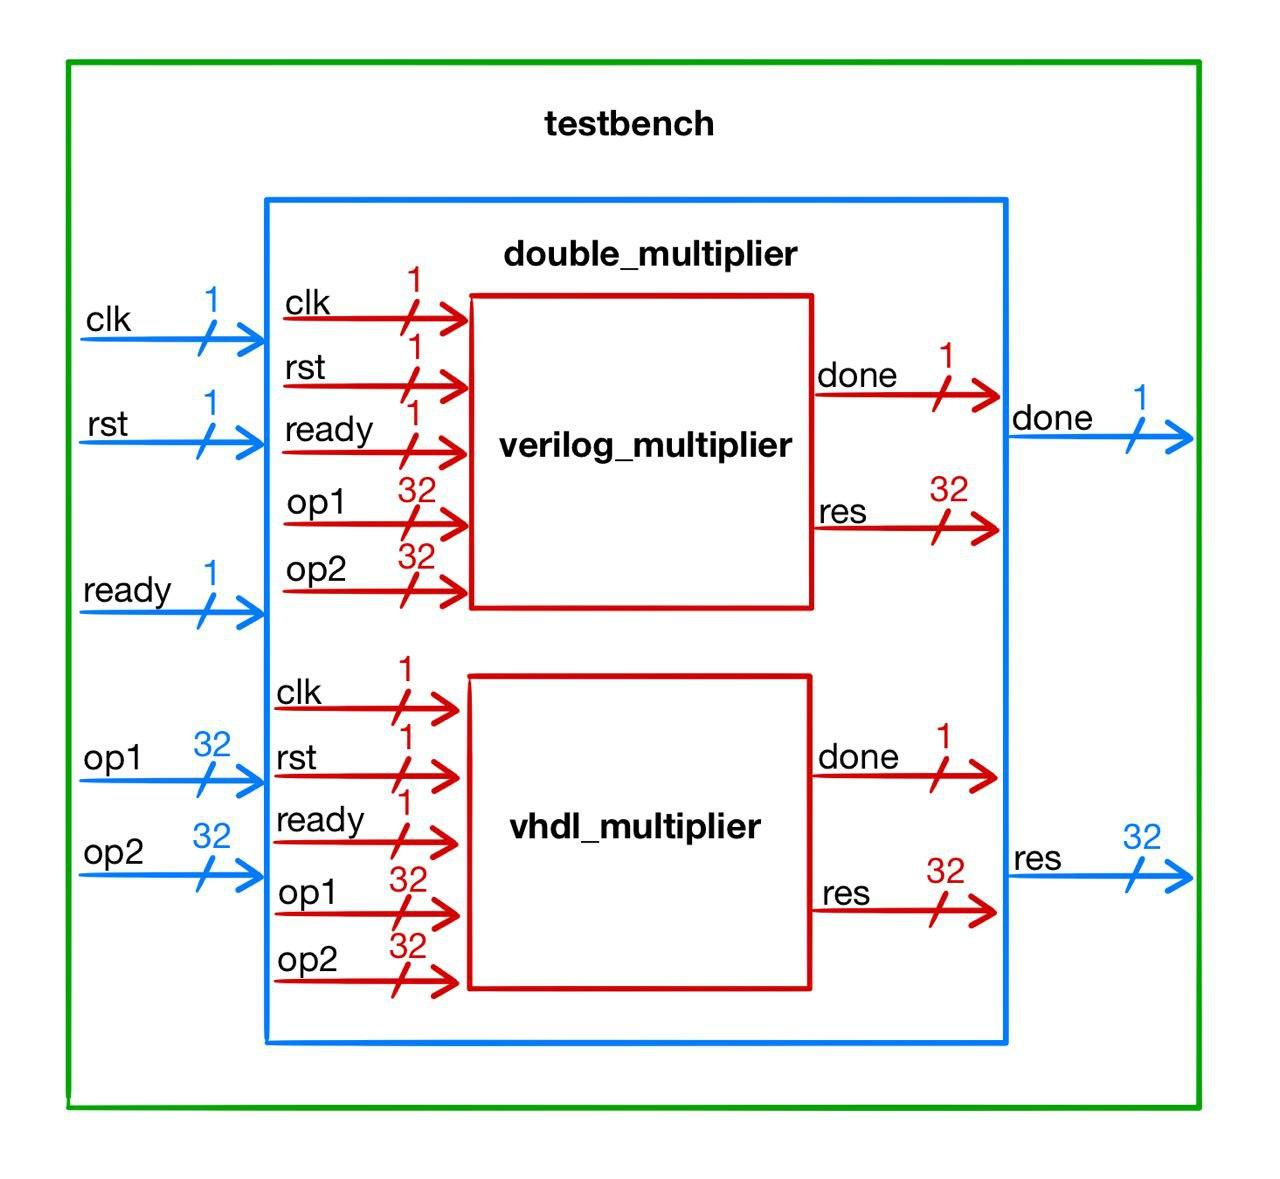
\includegraphics[width=0.8\linewidth]{figures/architettura}
    \caption{Architettura RTL}
    \label{fig:Architettura}
\end{figure}
Le FSMD realizzate usano tutte due processi:
\begin{itemize}
    \item \textbf{fsm:} processo asincrono col compito di calcolare e aggiornare lo stato prossimo.
    \item \textbf{datapath:} processo sincrono che ha il compito di aggiornare lo stato attuale ed elaborare gli output. Esso viene però attivato asincronamente dal fronte di salita del reset al fine di riportare lo stato a quello iniziale.
\end{itemize}


\subsection{multiplier}
Questo componente esegue la moltiplicazione tra numeri floating point a precisione singola.
\\L'interfaccia è mostrata in figura \ref{fig:Architettura}:
\begin{itemize}
    \item \textbf{op1} (32 bit input): primo operando.
    \item \textbf{op2} (32 bit input): secondo operando.
    \item \textbf{clk} (1 bit input): segnale di clock.
    \item \textbf{rst} (1 bit input): segnale di reset. Riporta il sistema allo stato iniziale.
    \item \textbf{ready} (1 bit input): segnale che permette al sistema di uscire dallo stato iniziale. Nello specifico indica che al prossimo fronte di salita del clock \textit{op1} e \textit{op2} conterranno i valori degli operandi.
    \item \textbf{done} (1 bit output): segnale che indica che il valore su \textit{res} è il risultato.
    \item \textbf{res} (32 bit output): risultato.
\end{itemize}

Gli altri segnali intermedi utilizzati sono:
\begin{itemize}\item \textbf{STATE e NEXT\_STATE} (4 bit): rappresentano lo stato attuale e lo stato prossimo.
    \item \textbf{esp\_tmp} (10 bit): permette di eseguire le operazioni per ricavare l'esponente finale senza perdere informazioni.
    \item \textbf{mant\_tmp} (48 bit): permette di eseguire le operazioni per ricavare la mantissa finale senza perdere informazioni.
    \item \textbf{sign1, sign2} (1 bit): rappresentano il segno dei due operandi.
    \item \textbf{esp1, esp2} (8 bit): rappresentano gli esponenti dei due operandi
    \item \textbf{mant1, mant2} (24 bit): rappresentano le mantisse dei due operandi. Esse presentano anche il bit omesso che sarà 1 nel caso di operandi normalizzati, 0 altrimenti.
\end{itemize}


L'algoritmo della moltiplicazione è descritto grazie alla EFSM [Figura \ref{fig:EFSM_MULT}] la quale è formata 19 stati:
\begin{itemize}
    \item \textbf{ST\_START:} stato di partenza. Qui vengono resettati i segnali interni e gli output a zero. In caso di segnale \textit{reset} a 1 si torna in questo stato. In caso di segnale \textit{ready} a 1 si passa a \textit{ST\_INIT}.
    \item \textbf{ST\_INIT:} qui vengono estrapolate le informazioni degli operandi di segno, esponente e mantissa la quale presenta anche il bit 24 a 1 (quello omesso nei 32 bit). Qui avviene anche la valutazione dei casi speciali, ovvero la generazione di NaN, $\infty$, 0, numeri subnormali che porterà nei rispetti stati. In caso il numero sia normalizzato si va allo stato \textit{ST\_ELAB}.
    \item \textbf{ST\_SNAN1:} si arriva a questo stato se il primo operando è un Signal NaN. In concordanza col metodo di testing e con l'articolo \cite{IEEE754Note}: ``Un signal NaN può essere copiato senza problemi, ma qualsiasi altra operazione è invalida e deve essere intercettata o prodotto un Nan non signal''. Quindi viene riscritto su \textit{res} il valore di \textit{op1} con il bit più significativo della mantissa a 1. Poi si passa a \textit{ST\_FINISH}.
    \item \textbf{ST\_SNAN2:} si arriva a questo stato se il secondo operando è un Signal NaN. Analogamente allo stato \textit{ST\_SNAN1}, viene riscritto su \textit{res} il valore di \textit{op2} con il bit più significativo della mantissa a 1. Poi si passa a \textit{ST\_FINISH}. In caso ci siano due SNAN come operandi si entra lo stesso in questo stato.
    \item \textbf{ST\_QNAN:} si arriva a questo stato se gli operandi sono 0 e $\infty$. In questo caso i primi 10 bit di \textit{res} sono posti a 1 e gli altri a 0. Poi si passa a \textit{ST\_FINISH}.
    \item \textbf{ST\_ZERO:} si arriva a questo stato se un operando è 0 e l'altro non è $\infty$. In questo caso il bit più significativo di \textit{res} è dato dallo xor del segno dei due operandi e gli altri bit sono posti a 0. Poi si passa a \textit{ST\_FINISH}.
    \item \textbf{ST\_INF:} si arriva a questo stato se un operando è $\infty$ e l'altro non è 0. In questo caso il bit più significativo di \textit{res} è dato dallo xor del segno, quelli dell'esponente sono posti tutti a 1 e quelli della mantissa a 0. Poi si passa a \textit{ST\_FINISH}.
    \item \textbf{ST\_ADJ1:} si arriva a questo stato se il primo operando è un numero subnormale e l'altro è normalizzato. In questo caso si pone il bit 24 di \textit{mant1} a 0 ed \textit{exp1} uguale a 1 perchè $1-127=-126$ cioè il valore corretto in caso di numero subnormale. Questa scelta è stata fatta per utilizzare lo stato \textit{ST\_ELAB} indipendentemente che il numero fosse normalizzato o subnormalizzato. Poi si passa a \textit{ST\_ELAB}.
    \item \textbf{ST\_ADJ2:} analogo a \textit{ST\_ADJ2} ma qui è \textit{op2} subnormale.
    \item \textbf{ST\_ADJ3:} analogo a \textit{ST\_ADJ1} e \textit{ST\_ADJ2} ma qui entrambi gli operandi sono subnormali.
    \item \textbf{ST\_ELAB:} qui viene ricavato l'esponente temporaneo come $exp\_tmp = exp1 + exp2 - 127$. Si sottrae 127 perchè altrimenti \textit{exp\_tmp} avrebbe sommato un bias di $127+127$. Viene anche ricavata la mantissa temporanea come $mant\_tmp = mant1 * mant2$. Poi si passa a \textit{ST\_SHIFTR} se il bit più significativo di \textit{mant\_tmp} vale 1, a \textit{ST\_SHIFTL} se i due bit più significativi sono "00" oppure \textit{ST\_CHECK} se sono "01".
    \item \textbf{ST\_SHIFTR:} qui si esegue lo shift a destra di \textit{mant\_tmp} per portarla nella forma 1.x, con conseguente incremento di \textit{exp\_tmp}. Poi si passa a \textit{ST\_CHECK}.
    \item \textbf{ST\_SHIFTL:} qui si esegue lo shift a sinistra di \textit{mant\_tmp} nella speranza di portarla nella forma 1.x, con conseguente decremento di \textit{exp\_tmp}. Poi si passa a \textit{ST\_NORM}.
    \item \textbf{ST\_NORM:} se \textit{mant\_tmp} è diventato nella forma 1.x allora si passa a \textit{ST\_CHECK}. Se \textit{exp\_tmp} è maggiore di 0 allora c'è ancora speranza di riuscire a ottenere un numero nella forma 1.x valido e quindi si passa a \textit{ST\_SHIFTL}, altrimenti si passa a \textit{ST\_CHECK} per valutare se è possibile rappresentare il risultato con un numero subnormale.
    \item \textbf{ST\_CHECK:} qui si controlla ciò che si è ottenuto dalle elaborazioni precedenti. Se \textit{exp\_tmp} ha tutti i bit a zero allora il numero è subnormale e si passa a \textit{ST\_SUBNORM}. Se \textit{exp\_tmp} ha i due bit più significativi a "01" allora c'è stato overflow e si passa a \textit{ST\_INF}. Se \textit{exp\_tmp} ha i due bit più significativi a "00" e il bit 22 di \textit{mant\_tmp} a 0 allora il risultato è un numero normalizzato e si passa a \textit{ST\_WRITE}. Se \textit{exp\_tmp} ha i due bit più significativi a "00" e il bit 22 di \textit{mant\_tmp} a 1 allora c'è bisogno di arrontare la mantissa e si passa a \textit{ST\_ROUND}. Se il bit più significativo di \textit{exp\_tmp} è 1 e la somma dell'esponente temporaneo con 48 (cioè in) è maggiore o uguale a 0 allora il risultato è rappresentabile con un numero subnormale, ma non è ancora pronto quindi si passa a \textit{ST\_SHIFTR} per portarlo alla forma giusta. Se il bit più significativo di \textit{exp\_tmp} è 1 e la somma dell'esponente temporaneo con 48 è minore di 0 allora si è verificato un underflow e si passa a \textit{ST\_ZERO}.
    \item \textbf{ST\_SUBNORM:} si arriva a questo stato quando il risultato è un numero subnormale. Il risultato però per essere pronto deve eseguire un ulteriore shift a destra della \textit{mant\_tmp}. Di conseguenza anche \textit{exp\_tmp} dovrebbe essere incrementato diventanto 1 però complementarmente a quanto accade negli stati \textit{ST\_ADJ1}, \textit{ST\_ADJ2}, \textit{ST\_ADJ3} si lascia l'esponente a zero. Poi si passa a \textit{ST\_WRITE}.
    \item \textbf{ST\_ROUND:} qui avviene l'arrotondamento della mantissa, il quale avviene solo se il bit a destra del punto di taglio di \textit{mant\_tmp} è 1. In questo caso si incrementa di 1 la parte a sinistra del punto di taglio della mantissa temporanea. nel caso in cui questo incremento faccia diventare il bit più significivo di \textit{mant\_tmp} a 1 si passa a \textit{ST\_SHIFTR} altrimenti si prosegue in \textit{ST\_WRITE}.
    \item \textbf{ST\_WRITE:} qui si assembla il risultato finale \textit{res}. In particolare il segno è dato dallo xor fra il segno degli operandi, l'esponente è dato da \textit{exp\_tmp} senza i due bit più significativi e la mantissa da \textit{mant\_tmp} senza i due bit più significativi e con solo i 23 successivi.
    \item \textbf{ST\_FINISH:} qui si pone il \textit{done} a 1.
\end{itemize}


\subsection{double\_multiplier}
Questo componente esegue due moltiplicazioni tra numeri floating point a precisione singola.
\\L'interfaccia è mostrata in figura \ref{fig:Architettura}:
\begin{itemize}
    \item \textbf{op1} (32 bit input): primo operando.
    \item \textbf{op2} (32 bit input): secondo operando.
    \item \textbf{clk} (1 bit input): segnale di clock.
    \item \textbf{rst} (1 bit input): segnale di reset. Riporta il sistema allo stato iniziale.
    \item \textbf{ready} (1 bit input): segnale che permette al sistema di uscire dallo stato iniziale. Nello specifico indica che al prossimo fronte di salita del clock \textit{op1} e \textit{op2} conterranno i valori degli operandi per la prima moltiplicazione e in quello successivo ci saranno quelli per la seconda moltiplicazione.
    \item \textbf{done} (1 bit output): segnale che indica che il valore su \textit{res} è il risultato.
    \item \textbf{res} (32 bit output): risultato.
\end{itemize}

Gli altri segnali intermedi utilizzati sono:
\begin{itemize}
    \item \textbf{ready1} (1 bit) segnale che pone il \textit{ready} del primo multiplier (quello in Verilog) a 1.
    \item \textbf{ready2} (1 bit) segnale che pone il \textit{ready} del secondo multiplier (quello in VHDL) a 1.
    \item \textbf{done1} (1 bit) segnale che indica che il valore su \textit{res1} è il risultato della prima moltiplicazione.
    \item \textbf{done2} (1 bit) segnale che indica che il valore su \textit{res2} è il risultato della seconda moltiplicazione.
\end{itemize}

L'algoritmo è descritto grazie alla EFSM [Figura \ref{fig:EFSM_DM}] la quale è formata 8 stati:
\begin{itemize}
    \item \textbf{ST\_START:} stato di partenza. Qui vengono resettati i segnali interni e gli output a zero. In caso di segnale \textit{reset} a 1 si torna in questo stato. In caso di segnale \textit{ready} a 1 si passa a \textit{ST\_RUN1}.
    \item \textbf{ST\_RUN1:} qui viene posto \textit{ready1} a 1, attivando quindi il primo moltiplicatore. Poi si passa a \textit{ST\_RUN2}.
    \item \textbf{ST\_RUN2:} qui viene posto \textit{ready2} a 1, attivando quindi il secondo moltiplicatore. Poi si passa a \textit{ST\_WAIT}.
    \item \textbf{ST\_WAIT:} qui vengono posti \textit{ready1} e \textit{ready2} uguali a 0. Si rimane in questo stato finchè \textit{done1} e \textit{done2} rimangono a 0. Se \textit{done1} diventa 1 allora si passa a \textit{ST\_WAIT2}, se \textit{done2} diventa 1 allora si passa a \textit{ST\_WAIT1} e nel caso si attivino contemporaneamente allora si passa direttamente a \textit{ST\_RET1}.
    \item \textbf{ST\_WAIT1:} si resta qui finchè non finisce anche il primo moltiplicatore, cioè finchè \textit{ready1} è uguale a 0. Poi si passa a \textit{ST\_RET1}.
    \item \textbf{ST\_WAIT2:} si resta qui finchè non finisce anche il secondo moltiplicatore, cioè finchè \textit{ready2} è uguale a 0. Poi si passa a \textit{ST\_RET1}.
    \item \textbf{ST\_RET1:} pone \textit{done} uguale a 1 e \textit{res} uguale al risultato del primo moltiplicatore cioè \textit{res1}. Poi si passa a \textit{ST\_RET2}.
    \item \textbf{ST\_RET2:} pone \textit{res} uguale al risultato del secondo moltiplicatore cioè \textit{res2} e ritorna allo stato iniziale.
\end{itemize}


\subsection{testbench}
Questo componente è un test automatizzato che incorpora il \textit{double\_multiplier} come mostrato in figura \ref{fig:Architettura}.
\\La versione in Verilog ha il compiti di verificare:
\begin{itemize}
    \item che i sottocomponenti in Verilog e VHDL diano gli stessi risultati.
    \item che il \textit{double\_multiplier} esegue correttamente due moltiplicazioni con operandi diversi.
    \item che vengano provati per ogni nodo della EFSM tutti gli archi.
\end{itemize}
La versione in SystemC sono state messe a disposizione tre thread (da attivare togliendo i commenti del costruttore del \textit{TestbenchModule} nel file testbench\_RTL.cc):
\begin{itemize}
    \item \textbf{target\_test:} testa l'esecuzione di due specifici operandi scelti da una lista.
    \item \textbf{full\_target\_test:} testa tutti gli elementi della lista, i quali sono scelti appositamente per provare tutti gli archi di ogni nodo della EFSM.
    \item \textbf{rnd\_test:} testa l'esecuzione del \textit{double\_multiplier} con valori generati randomicamente.
\end{itemize}
Per i testbench in entrambi i linguaggi è stato usato un array di bits contenenti gli inputs da testare. In SystemC sono state create due funzioni ausiliarie ``binary\_to\_float()'' e ``float\_to\_binary()'' per confrontare il risultato ottenuto dal \textit{double\_multiplier} con quelli ottenuti da una semplice moltiplicazione in c++. I risultati ottenuti sono stati interiti nell'array del testbench in Verilog per realizzare il test automatico.



\section{risultati}

\subsection{Simulazioni con script TCL}
Dopo aver realizzato il \textit{multiplier} in Verilog, questo è stato subito testato con un semplice script TCL. In questo modo si è potuto controllare facilmente che il componente esegua i passaggi aspettati. In particolare sono stati ricercati e provati gli input necessari a testare ogni arco della EFSM. Nel file ``/stimuli/multiplier.tcl'' si possono vedere i vari input testati, con gli stati percorsi e il risultato obiettivo ricavato grazie alle funzioni ausiliarie del testbench SystemC. Nelle figure \ref{fig:SIM_MULT_VERILOG} e \ref{fig:SIM_MULT_VHDL} si possono guardare le simulazioni dei moltiplicatori con lo script TCL.
\\Lo script TCL per il \textit{double\_multiplier} analogamente è servito a controllare il corretto funzionamento del componente, in particolare che i moltiplicatori ricevessero i giusti input. In figura \ref{fig:SIM_DM} si può guardare la simulazione con lo script TCL.


\subsection{Simulazione con testbench in Verilog}
I test con gli script TCL sono serviti principalmente a controllare nel dettaglio il comporamento dei componenti e a ricavare gli input per questo testbench.
\\Questo test ha due compiti:
\begin{itemize}
    \item Verificare che il \textit{multiplier} VHDL dia gli stessi valori di quello Verilog.
    \item Verificare che il \textit{double\_multiplier} esegua correttamente due moltiplicazioni diverse.
\end{itemize}
In particolare è utilizzato per capire in modo automatico se i componenti fanno ciò che si aspetta, restituendo OK in caso il test sia andato a buon fine, mentre FAIL con il risultato ottenuto e quello corretto in caso di errore.
In figura \ref{fig:SIM_TB_BH} si può vedere un pezzo della simulazione con questo testbench a livello Behavioral e in figura \ref{fig:SIM_TB_BH_RES} i risultati ottenuti.
In figura \ref{fig:SIM_TB_TIM} si può vedere un pezzo della ``post-implementation timing simulation'' cioè la simulazione più simile al comportamento effettivo sulla fpga e in figura \ref{fig:SIM_TB_TIM_RES} i risultati ottenuti.


\subsection{Simulazione con testbench in SystemC}
In questo tesbench sono state messe a disposizione tre tipi di test differenti.
\\Il primo, mostrato in figura \ref{fig:SIM_SC_TARGET} ha lo scopo di testare semplicemente due input. Questo è stato utilizzato per ricavare il risultato in bit da utilizzare per il testbench in Verilog e analogamente allo script TCL, permette di controllare che il sistema percorra gli stati corretti.
\\Il secondo, mostrato in figura \ref{fig:SIM_SC_FULL} è analogo al testbench in Verilog e testa tutti gli input selezionati appositamente e disposti in un array. Ha il compito di testare la correttezza del sistema con gli input ritenuti più significativi.
\\Il terzo, mostrato in figura \ref{fig:SIM_SC_RND} ha lo scopo di dare una maggiore sicurezza sulla correttezza del sistema e in particolare trovare operandi che causano moltiplicazioni errate, dovute a casi non tenuti in considerazione durante la progettazione della EFSM. Questo test ha portato più volte ad una modifica del EFSM, in particolare a causa dei numeri subnormali (come numeri normalizzati che creano subnormali, subnormali che creano underflow, ecc).
\\Come mostrato in figura \ref{fig:SIM_SC_ERROR} il test fallisce in alcuni casi a causa del metodo di arrotondamento utilizzato. Essendoci però più metodi di arrotondamento usabili nello standard, è stato deciso di lasciare quello utilizzato in quanto più semplice.


\subsection{Sintesi}
La sintesi è stata fatta per la scheda Pynq xc7z020clg400-1.
\\In figura \ref{fig:UTIL_SYNT_VERILOG} e \ref{fig:UTIL_IMPL_VERILOG} si possono vedere i valori di utilizzo delle risorse post-syntesis e post-implementation del \textit{verilog\_multiplier}. L'unica differenza fra le due sono le 4 LTU in meno dopo l'implementazione. In figura \ref{fig:TIMING_VERILOG} si possono vedere i risultati di timing.
\begin{figure}[!htb]
    \centering
    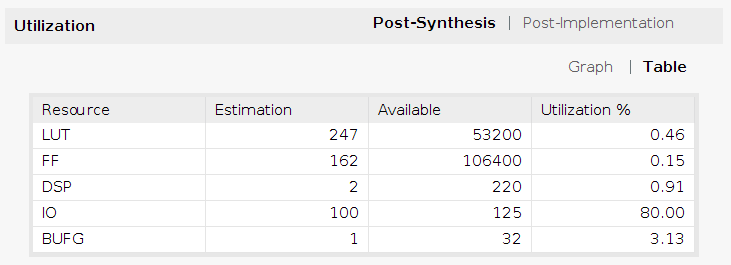
\includegraphics[width=0.9\linewidth]{figures/util_synt_verilog}
    \caption{Valori di utilizzo risorse post syntesis del \textit{verilog\_multiplier}}
    \label{fig:UTIL_SYNT_VERILOG}
\end{figure}
\begin{figure}[!htb]
    \centering
    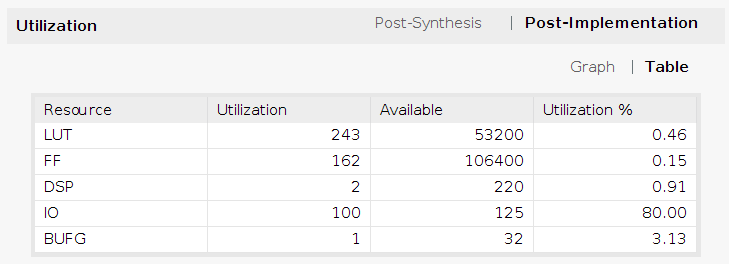
\includegraphics[width=0.9\linewidth]{figures/util_impl_verilog}
    \caption{valori di utilizzo risorse post implementation del \textit{verilog\_multiplier}}
    \label{fig:UTIL_IMPL_VERILOG}
\end{figure}
\begin{figure}[!htb]
    \centering
    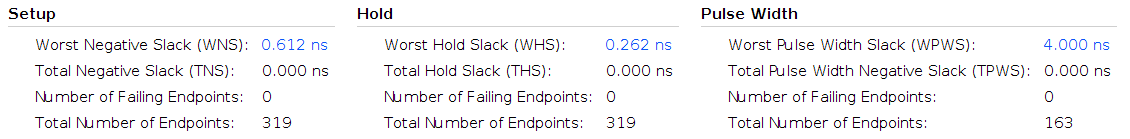
\includegraphics[width=0.9\linewidth]{figures/timing_verilog}
    \caption{Valori di timing del \textit{verilog\_multiplier}}
    \label{fig:TIMING_VERILOG}
\end{figure}

In figura \ref{fig:UTIL_SYNT_VHDL} e \ref{fig:UTIL_IMPL_VHDL} si possono vedere i valori di utilizzo delle risorse post-syntesis e post-implementation del \textit{vhdl\_multiplier}. L'unica differenza fra le due sono le 7 LTU in meno dopo l'implementazione. In figura \ref{fig:TIMING_VHDL} si possono vedere i risultati di timing.
\begin{figure}[!htb]
    \centering
    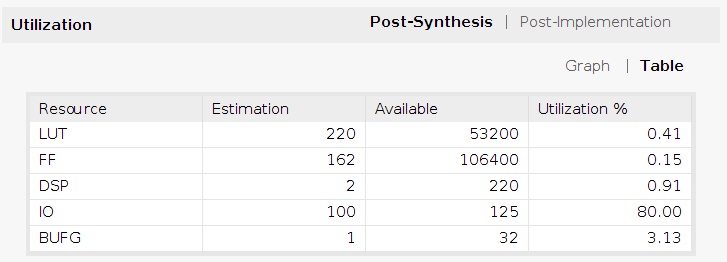
\includegraphics[width=0.9\linewidth]{figures/util_synt_vhdl}
    \caption{Valori di utilizzo risorse post syntesis del \textit{vhdl\_multiplier}}
    \label{fig:UTIL_SYNT_VHDL}
\end{figure}
\begin{figure}[!htb]
    \centering
    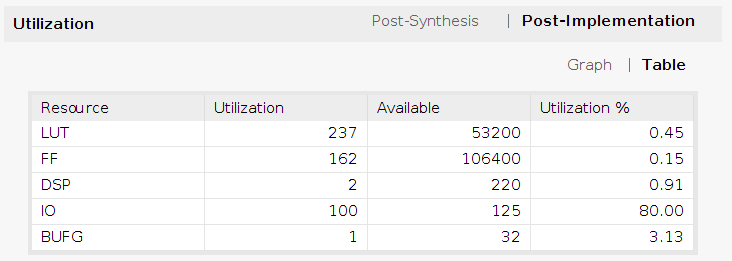
\includegraphics[width=0.9\linewidth]{figures/util_impl_vhdl}
    \caption{valori di utilizzo risorse post implementation del \textit{vhdl\_multiplier}}
    \label{fig:UTIL_IMPL_VHDL}
\end{figure}
\begin{figure}[!htb]
    \centering
    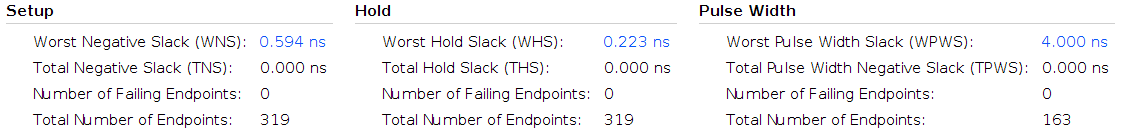
\includegraphics[width=0.9\linewidth]{figures/timing_vhdl}
    \caption{Valori di timing del \textit{vhdl\_multiplier}}
    \label{fig:TIMING_VHDL}
\end{figure}

In figura \ref{fig:UTIL_SYNT_DM} e \ref{fig:UTIL_IMPL_DM} si possono vedere i valori di utilizzo delle risorse post-syntesis e post-implementation del \textit{vhdl\_multiplier}. L'unica differenza fra le due sono le 7 LTU in meno dopo l'implementazione. In figura \ref{fig:TIMING_DM} si possono vedere i risultati di timing.
\begin{figure}[!htb]
    \centering
    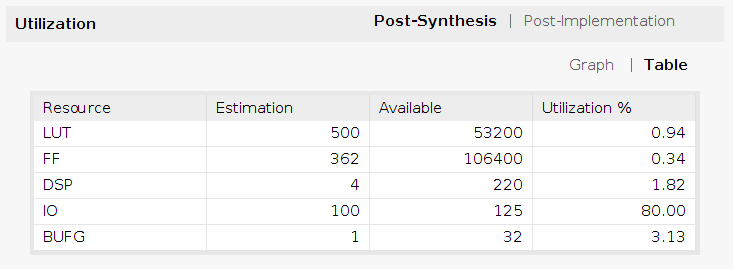
\includegraphics[width=0.9\linewidth]{figures/util_synt_dm}
    \caption{Valori di utilizzo risorse post syntesis del \textit{double\_multiplier}}
    \label{fig:UTIL_SYNT_DM}
\end{figure}
\begin{figure}[!htb]
    \centering
    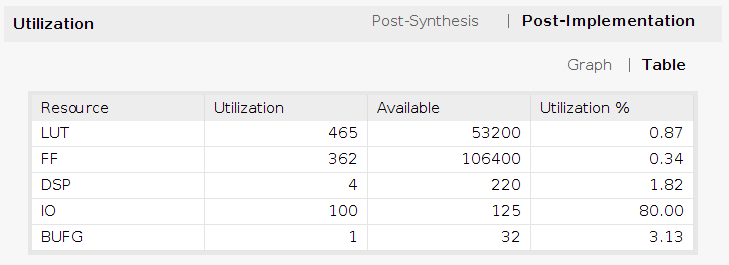
\includegraphics[width=0.9\linewidth]{figures/util_impl_dm}
    \caption{valori di utilizzo risorse post implementation del \textit{double\_multiplier}}
    \label{fig:UTIL_IMPL_DM}
\end{figure}
\begin{figure}[!htb]
    \centering
    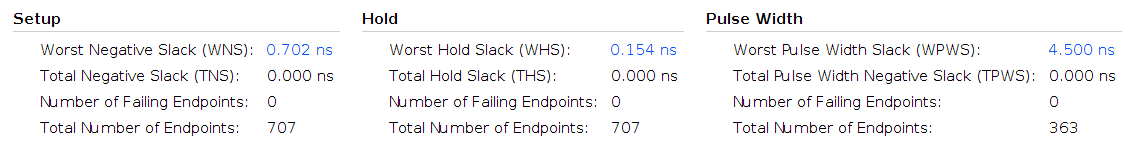
\includegraphics[width=0.9\linewidth]{figures/timing_dm}
    \caption{Valori di timing del \textit{double\_multiplier}}
    \label{fig:TIMING_DM}
\end{figure}

Si nota subito come la versione VDHL dia risultati migliori sia a livello di spazio che di tempo rispetto a quella in Verilog, ciò fa capire che la scelta del linguaggio non è indifferente dal punto di vista delle performante.
\\Il periodo di clock massimo raggiungibile prima che WNS diventi negativo (e che quindi vengano verificate violazioni) è 9ns, ma con questo valore la simulazione post-implementation del tempo da valori sbagliati. Per questo motivo è stato usato come periodo di clock minimo 10ns.
\\In figura \ref{fig:DEVICE} è possibile guardare la parte utilizzata della FPGA con il sistema realizzato, che come ci si aspettava è molto ridotta. Infine in figura \ref{fig:POWER_SUMMARY} e \ref{fig:POWER_ONCHIP} si possono vedere i valori di potenza.
\begin{figure}[!htb]
    \centering
    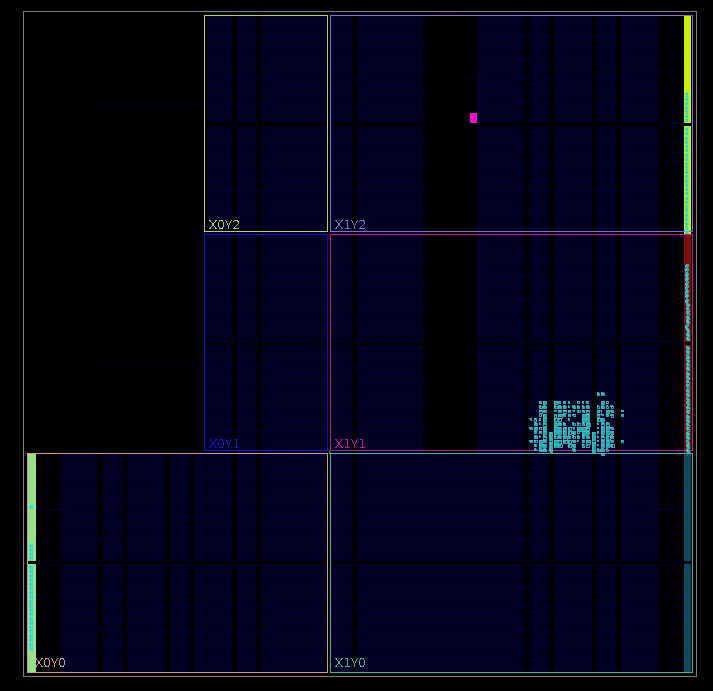
\includegraphics[width=0.9\linewidth]{figures/device_impl}
    \caption{valori di utilizzo risorse post implementation del \textit{double\_multiplier}}
    \label{fig:DEVICE}
\end{figure}
\begin{figure}[!htb]
    \centering
    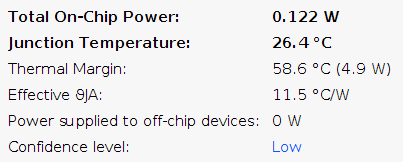
\includegraphics[width=0.9\linewidth]{figures/power_summary}
    \caption{Power summary}
    \label{fig:POWER_SUMMARY}
\end{figure}
\begin{figure}[!htb]
    \centering
    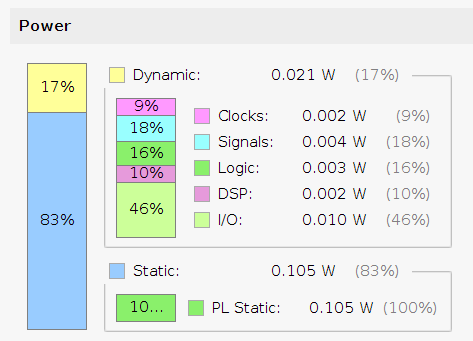
\includegraphics[width=0.9\linewidth]{figures/power_onChip}
    \caption{Power on-Chip}
    \label{fig:POWER_ONCHIP}
\end{figure}


\section{Conclusioni}

\nocite{*}
\bibliographystyle{IEEEtran}
\bibliography{biblio}
\appendix

\begin{figure*}[bt]
    \centering
    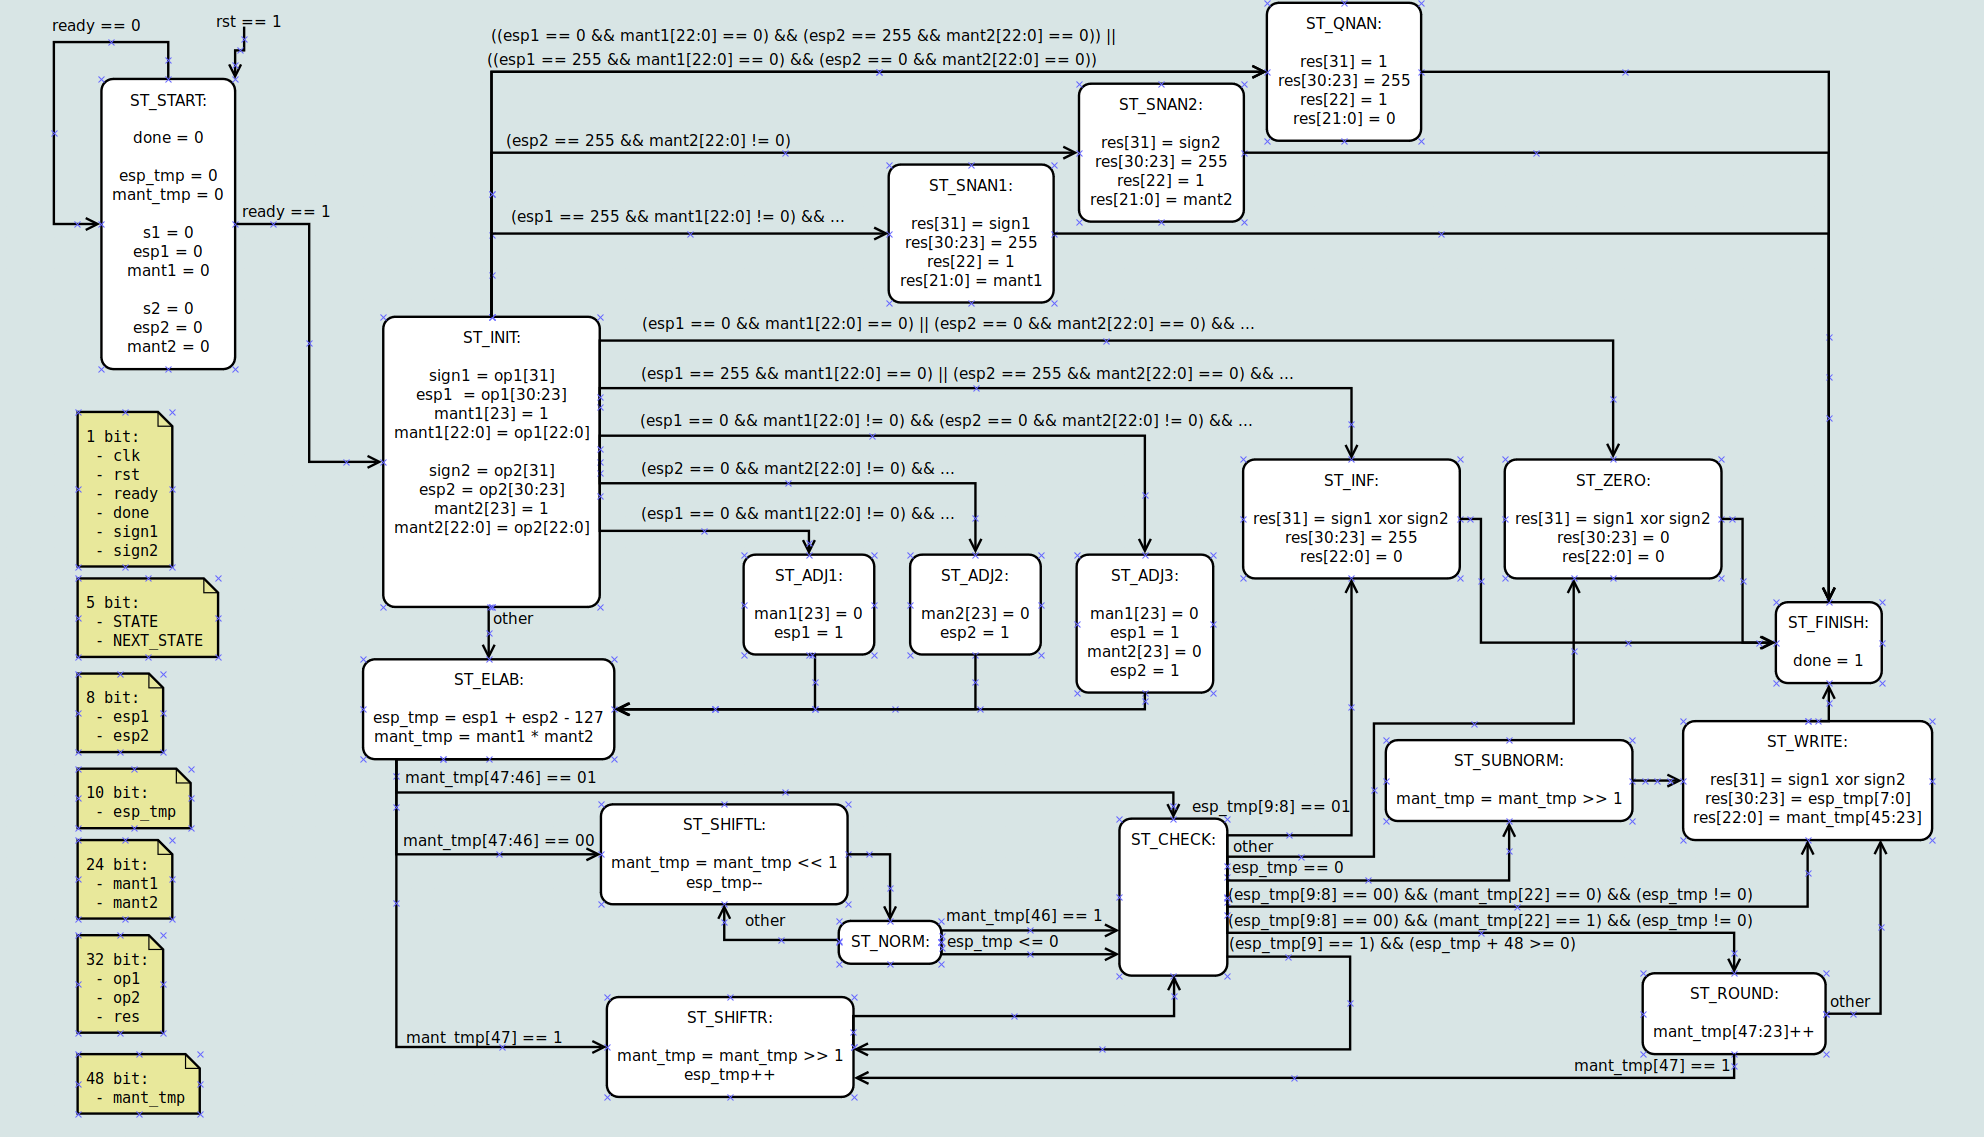
\includegraphics[width=\textwidth]{figures/EFSM_mult}
    \caption{EFSM del multiplier}
    \label{fig:EFSM_MULT}
\end{figure*}

\begin{figure*}[bt]
    \centering
    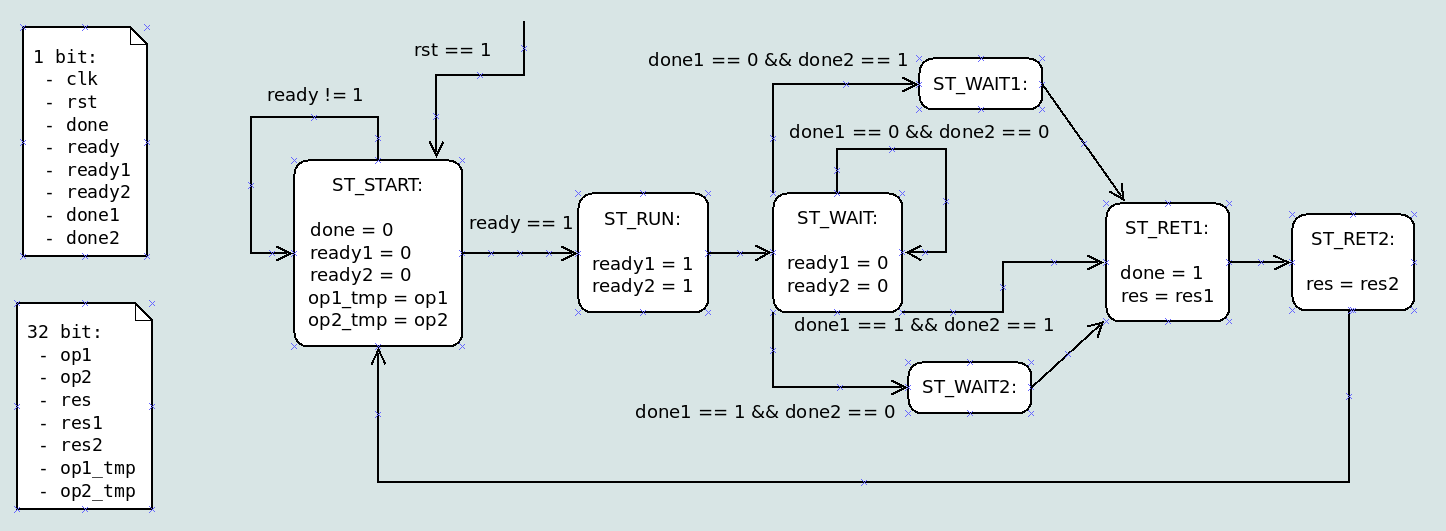
\includegraphics[width=\textwidth]{figures/EFSM_dm}
    \caption{EFSM del double\_multiplier}
    \label{fig:EFSM_DM}
\end{figure*}

\begin{figure*}[bt]
    \centering
    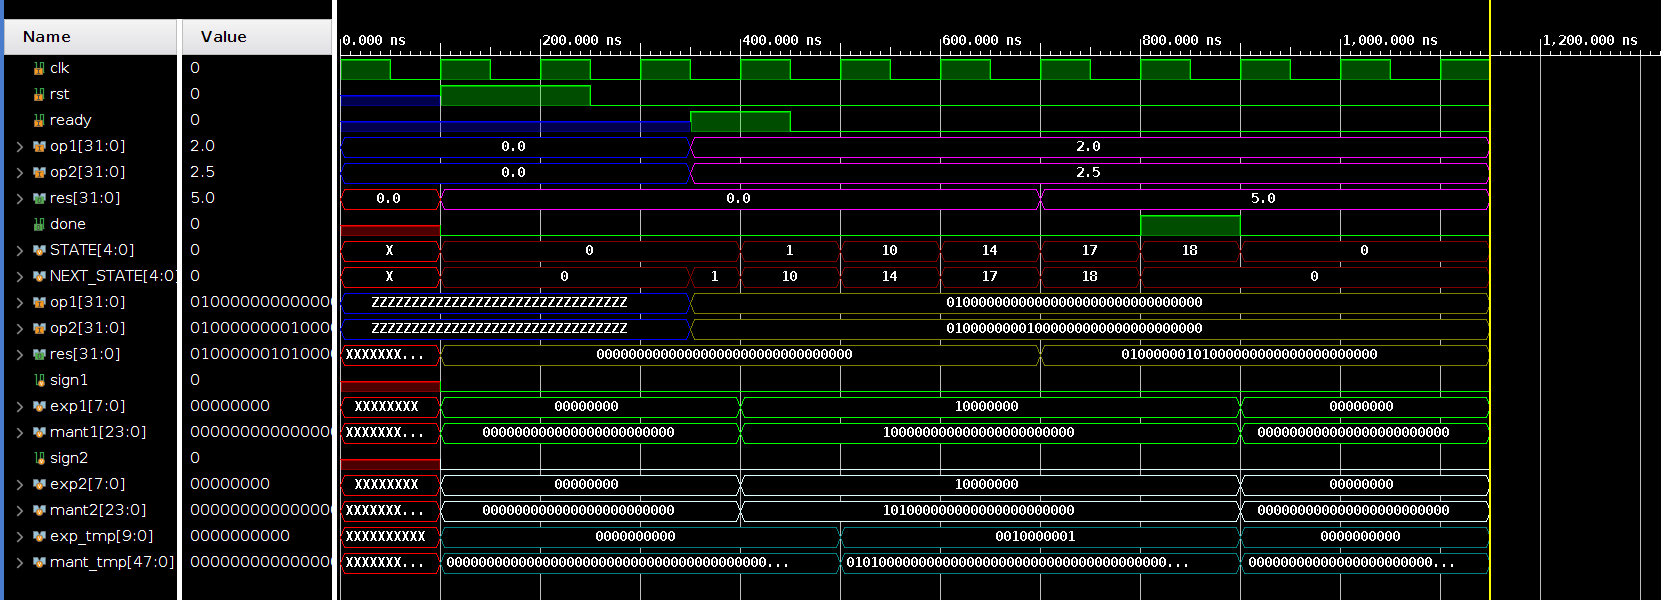
\includegraphics[width=\textwidth]{figures/sim_mult_verilog}
    \caption{Simulazione multiplier in Verilog con script TCL}
    \label{fig:SIM_MULT_VERILOG}
\end{figure*}

\begin{figure*}[bt]
    \centering
    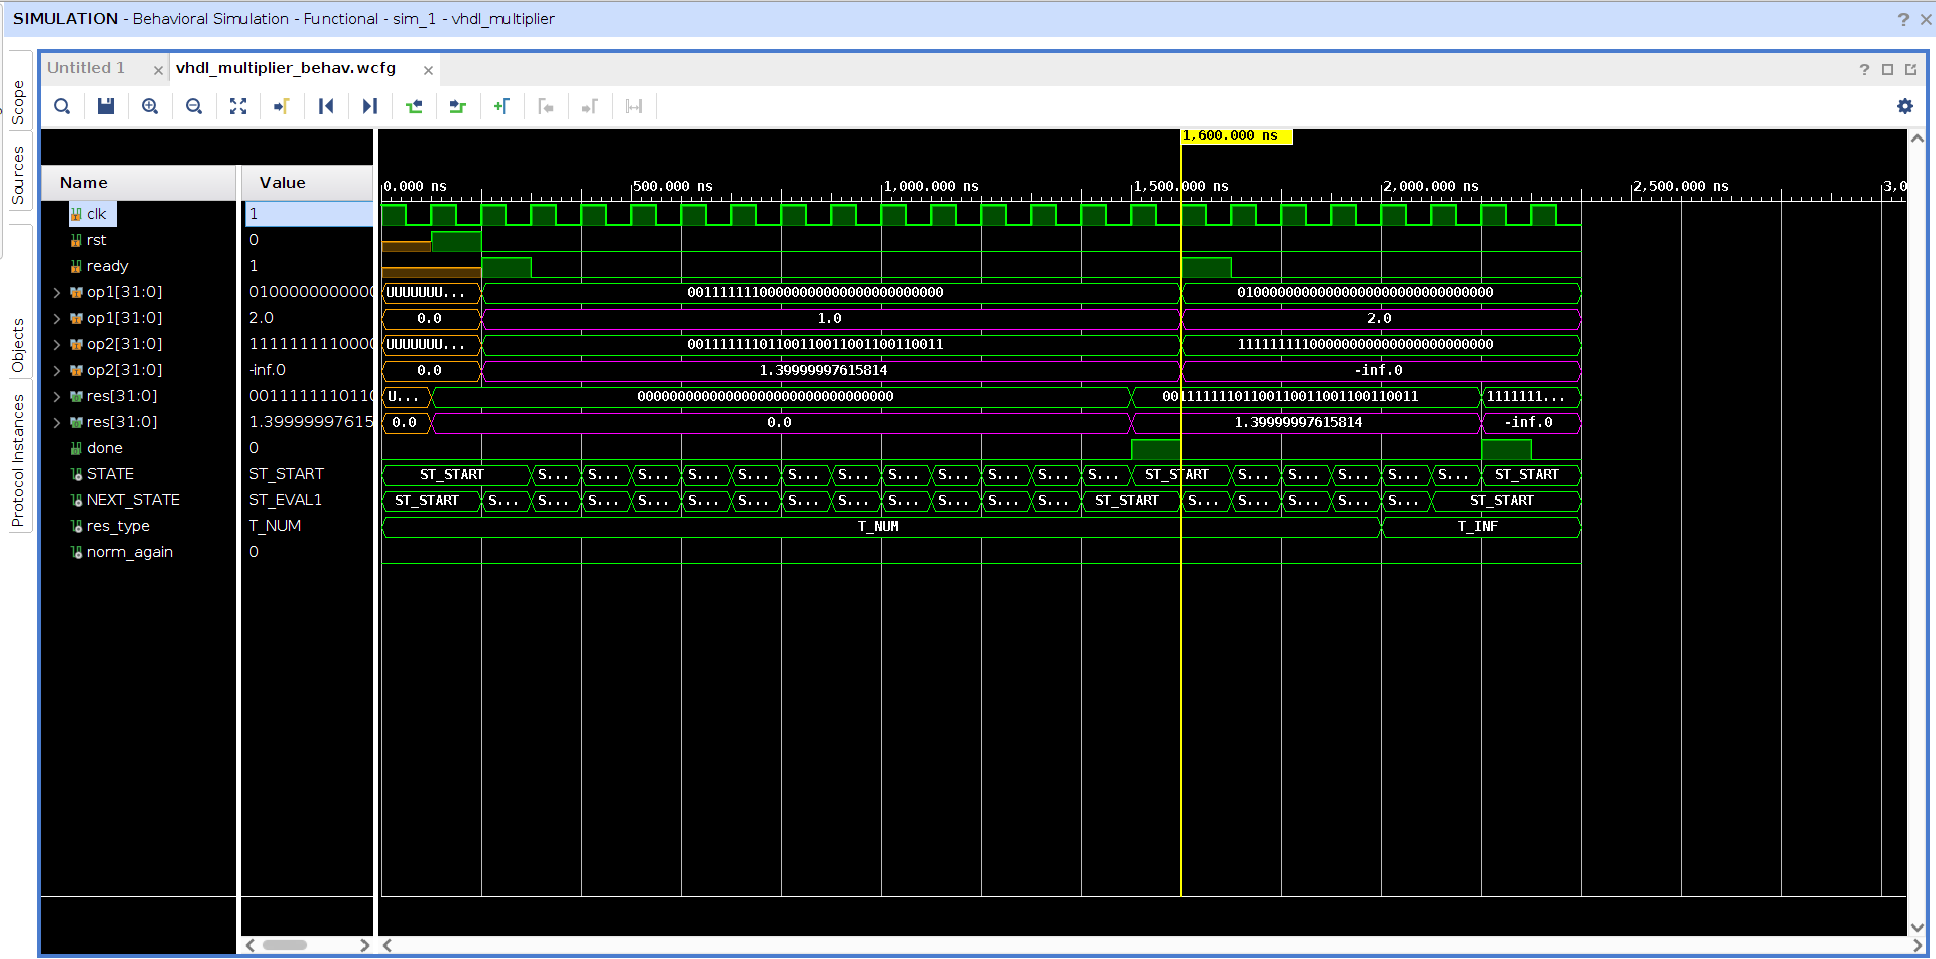
\includegraphics[width=\textwidth]{figures/sim_mult_vhdl}
    \caption{Simulazione multiplier in VHDL con script TCL}
    \label{fig:SIM_MULT_VHDL}
\end{figure*}

\begin{figure*}[bt]
    \centering
    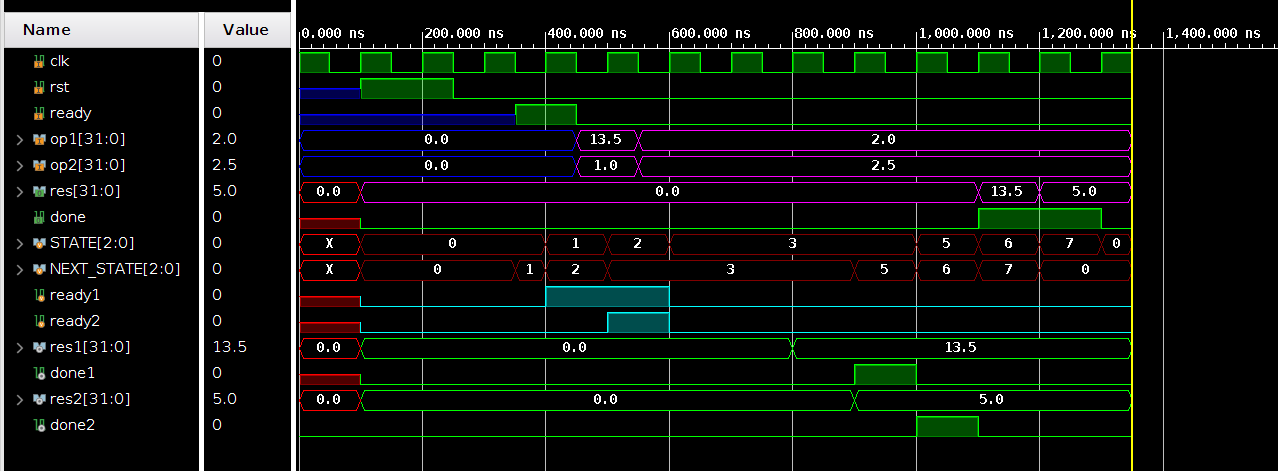
\includegraphics[width=\textwidth]{figures/sim_dm}
    \caption{Simulazione double\_multiplier in Verilog con script TCL}
    \label{fig:SIM_DM}
\end{figure*}

\begin{figure*}[bt]
    \centering
    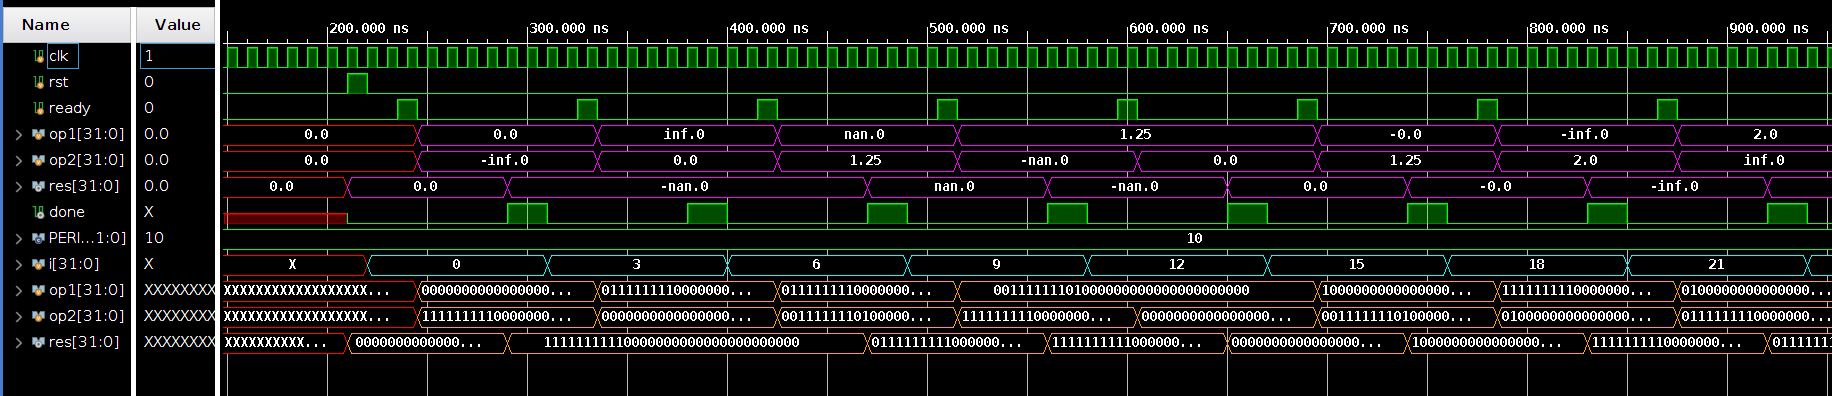
\includegraphics[width=\textwidth]{figures/sim_tb_bh}
    \caption{Behavioral simulation double\_multiplier in Verilog con testbench}
    \label{fig:SIM_TB_BH}
\end{figure*}

\begin{figure*}
    \centering
    \subfloat[VHDL vs Verilog]{{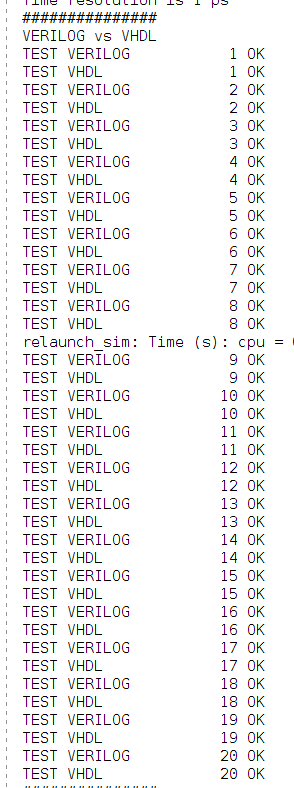
\includegraphics[width=0.3\textwidth]{figures/tb_bh1} }}
    \subfloat[VHDL and Verilog]{{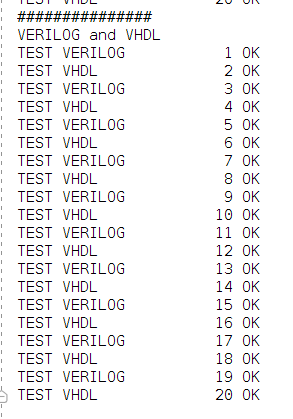
\includegraphics[width=0.3\textwidth]{figures/tb_bh2} }}
    \caption{Risultati testbench Behavioral}
    \label{fig:SIM_TB_BH_RES}
\end{figure*}

\begin{figure*}[bt]
    \centering
    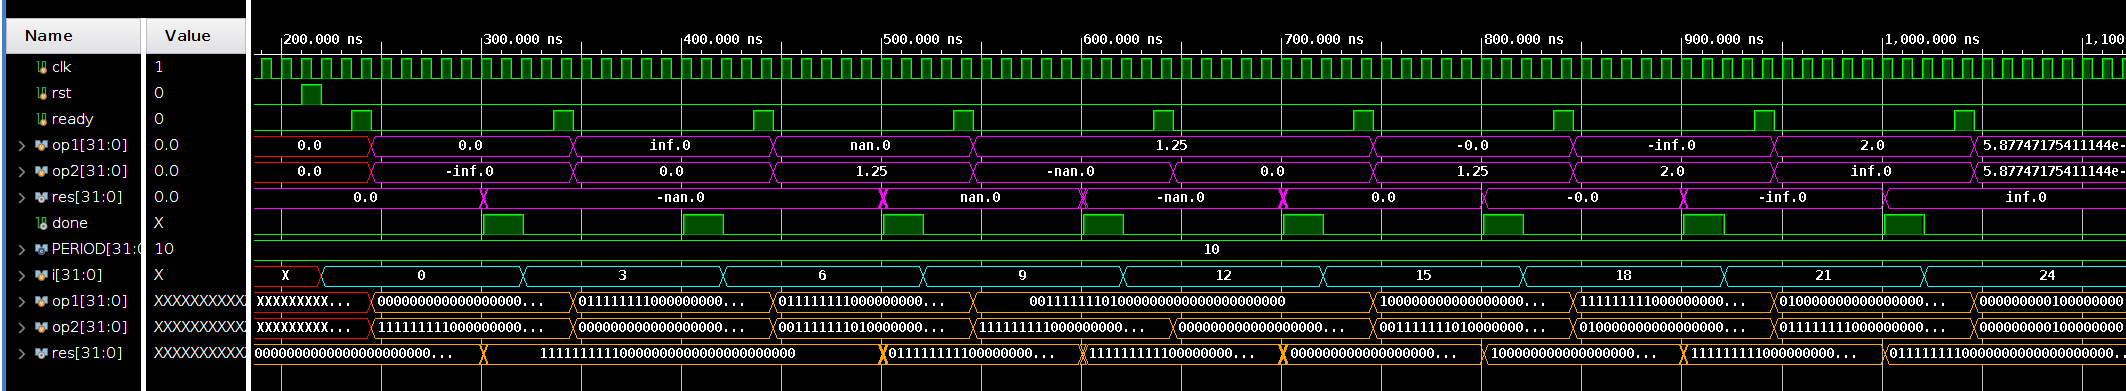
\includegraphics[width=\textwidth]{figures/sim_tb_tim}
    \caption{Post-Implementation Timing simulation double\_multiplier in Verilog con testbench}
    \label{fig:SIM_TB_TIM}
\end{figure*}
\begin{figure*}
    \centering
    \subfloat[VHDL vs Verilog]{{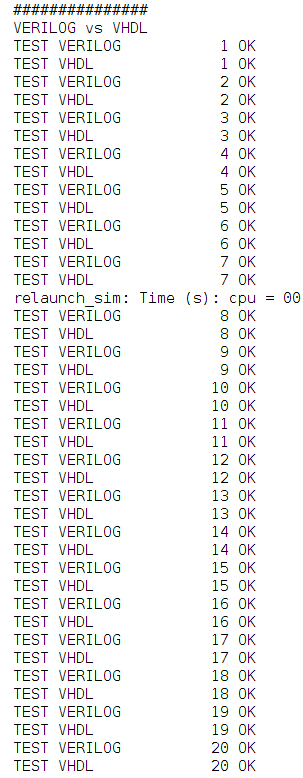
\includegraphics[width=0.3\textwidth]{figures/tb_tim1} }}
    \subfloat[VHDL and Verilog]{{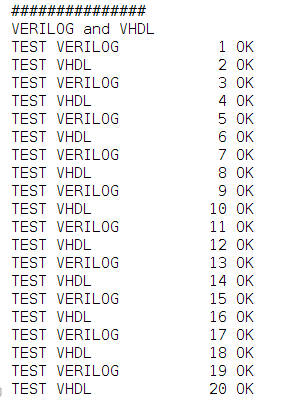
\includegraphics[width=0.3\textwidth]{figures/tb_tim2} }}
    \caption{Risultati testbench Post-Implementation}
    \label{fig:SIM_TB_TIM_RES}
\end{figure*}

\begin{figure*}[bt]
    \centering
    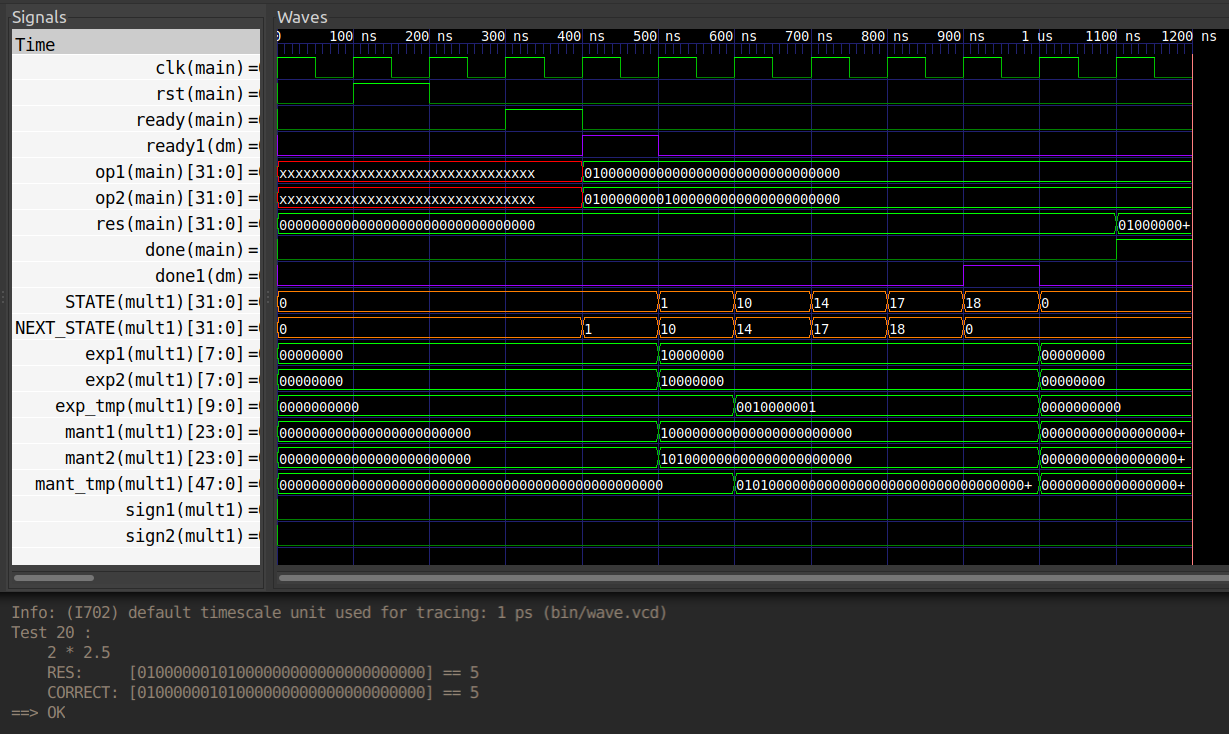
\includegraphics[width=\textwidth]{figures/sc_target}
    \caption{Simulazione double\_multiplier in SystemC con ``target test''}
    \label{fig:SIM_SC_TARGET}
\end{figure*}

\begin{figure*}[bt]
    \centering
    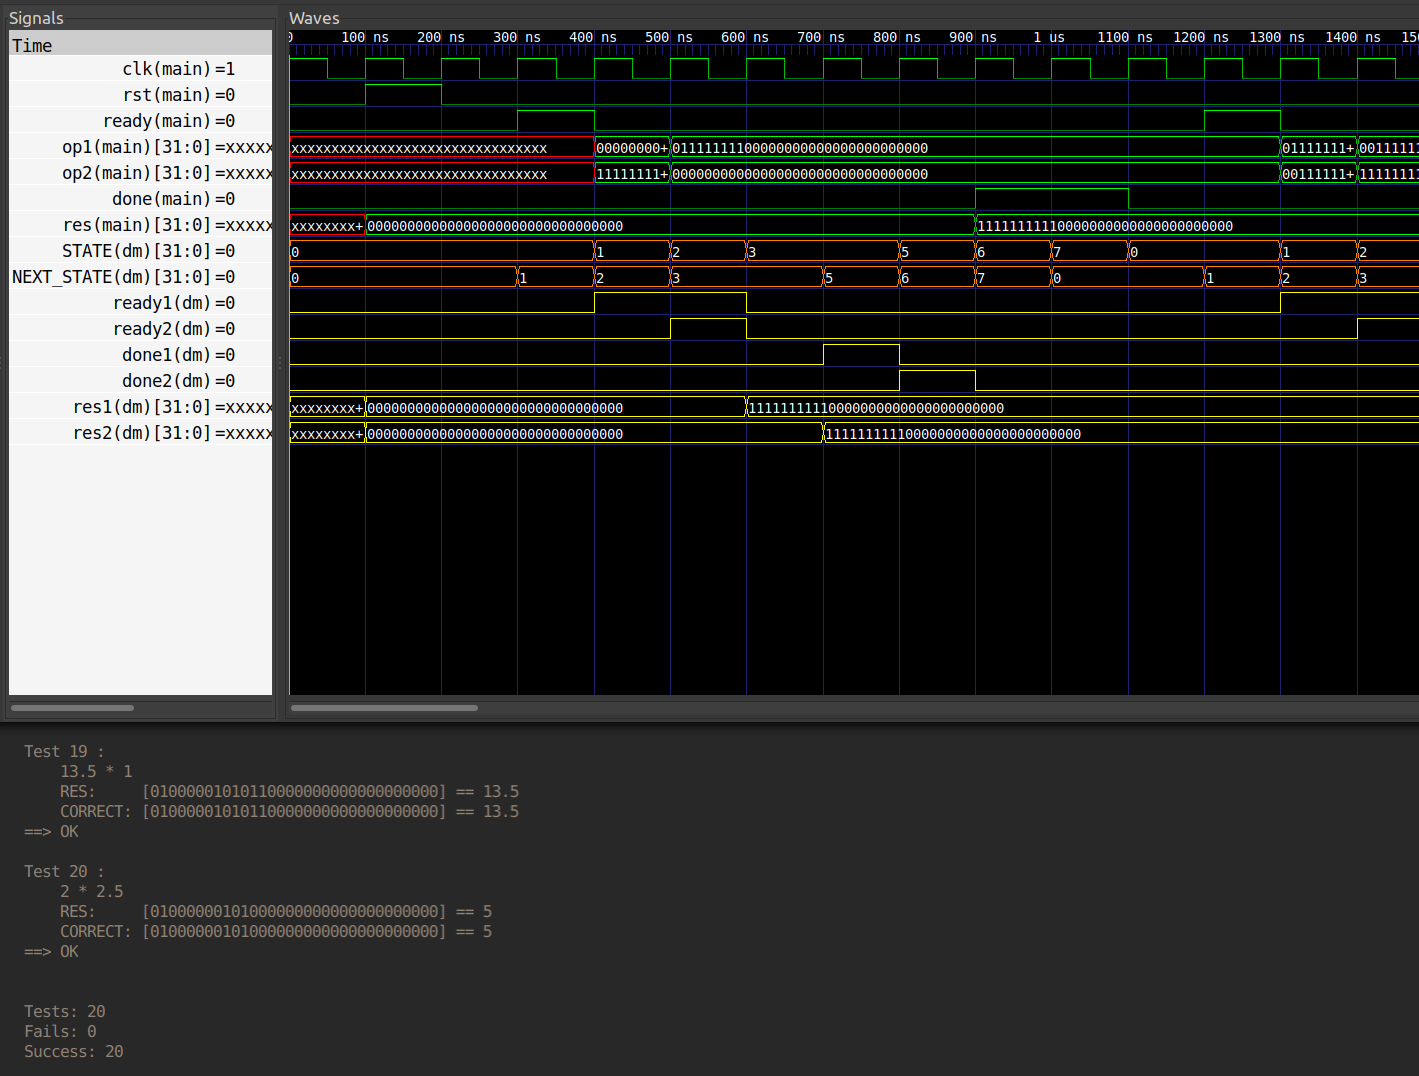
\includegraphics[width=\textwidth]{figures/sc_full}
    \caption{Simulazione double\_multiplier in SystemC con ``full target test''}
    \label{fig:SIM_SC_FULL}
\end{figure*}

\begin{figure*}[bt]
    \centering
    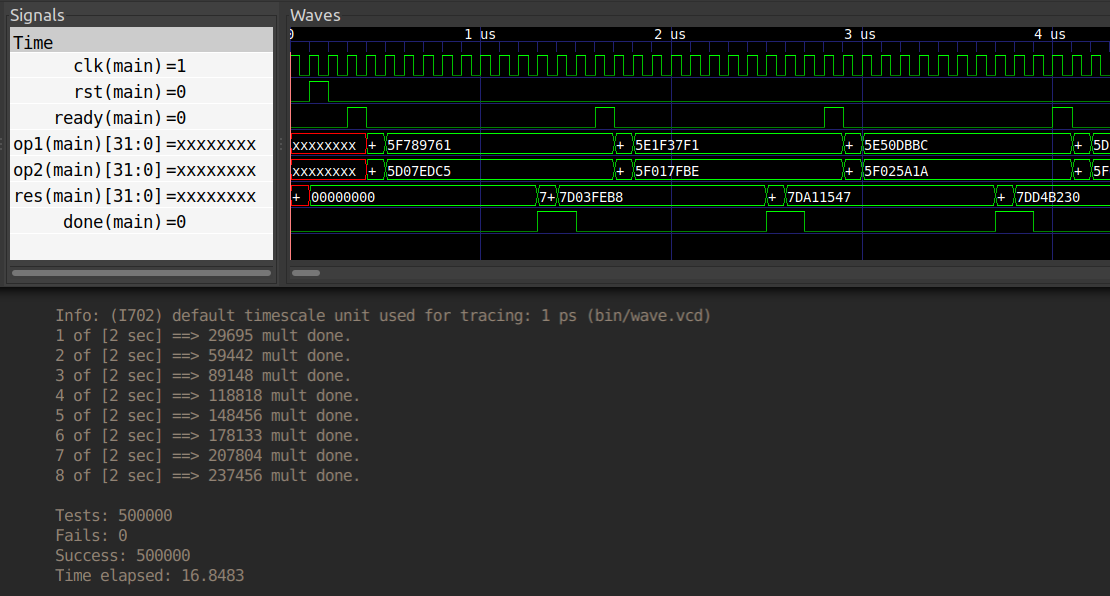
\includegraphics[width=\textwidth]{figures/sc_rnd}
    \caption{Simulazione double\_multiplier in SystemC con ``random test''}
    \label{fig:SIM_SC_RND}
\end{figure*}

\begin{figure*}[bt]
    \centering
    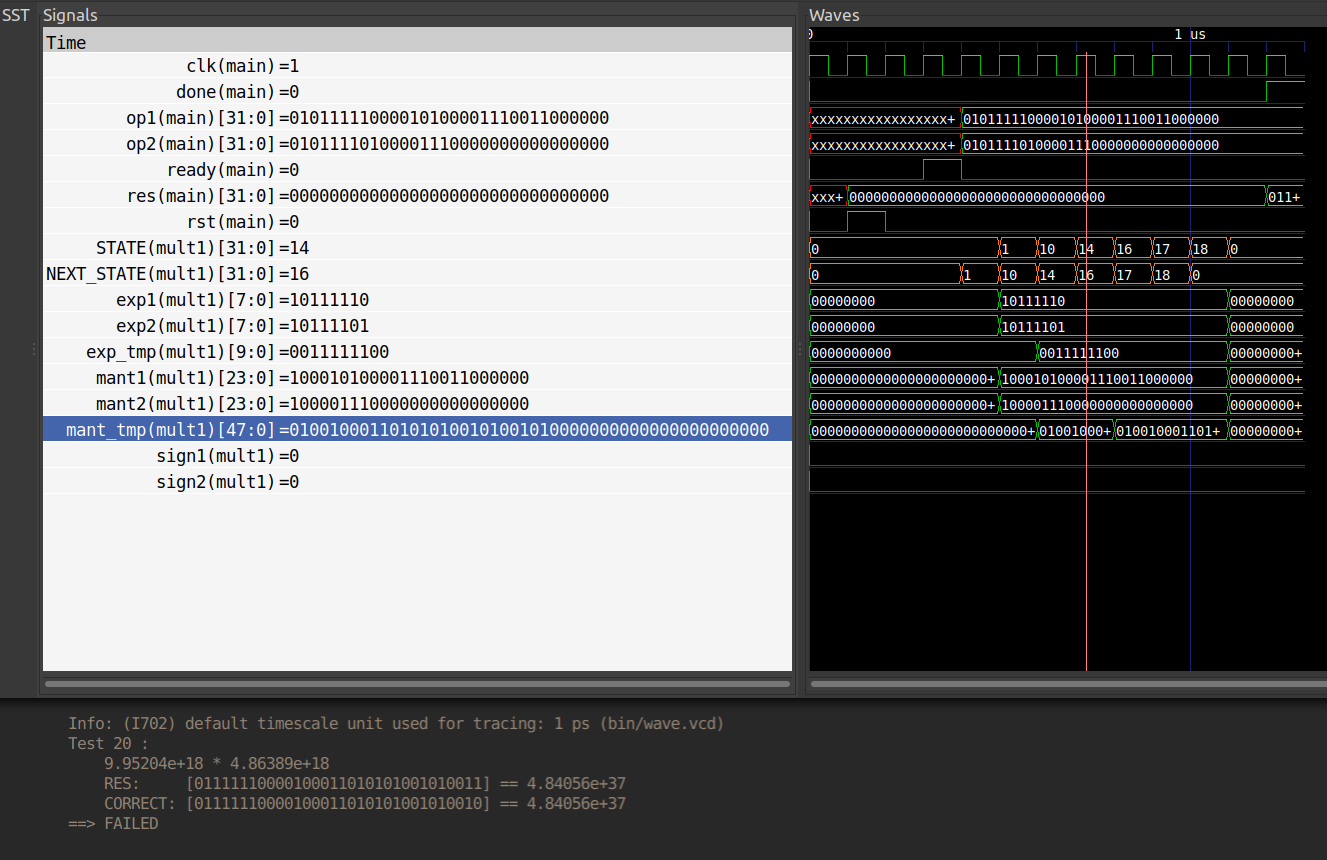
\includegraphics[width=\textwidth]{figures/sc_error}
    \caption{Simulazione double\_multiplier in SystemC con errore dovuto all'arrotondamento}
    \label{fig:SIM_SC_ERROR}
\end{figure*}


\end{document}